\chapter{Implementation}

\textbf{Author: } 

\section{Generating test data}
Good test data is of utmost importance in machine learning. The system can only know information that is depicted in the training data, which is why it is important to include as many aspects of the problem as possible in this data.

Since machine learning needs a lot of data in order to solve the given task it can be tiresome to generate and label all this data by hand. Therefore the authors decided to simulate the objects and the camera using a computer graphics modelling software called Blender.

Blender allows for relatively easy generation of training data by providing a Python API.

[TODO: Image camera setup, lightning, objects in Blender]

[TODO: Renders and labels for example objects]

\section{OpenCV}
OpenCV is a framework for image manipulation. Some of its use cases are changing the colour spectrum, filtering the image by colour and cropping images. The authors use OpenCV to test whether there are differences between filters for the images in the training data, for example greyscale images compared to coloured images.

[TODO: image manipulation und ...; aka besser beschreiben was OpenCV ist]

[TODO: wofür verwenden wir es? Ergebnisse zw. Graustufen und Farbbildern]

[TODO: Codebeispiele?]

\begin{figure}[h!]
	\centering
	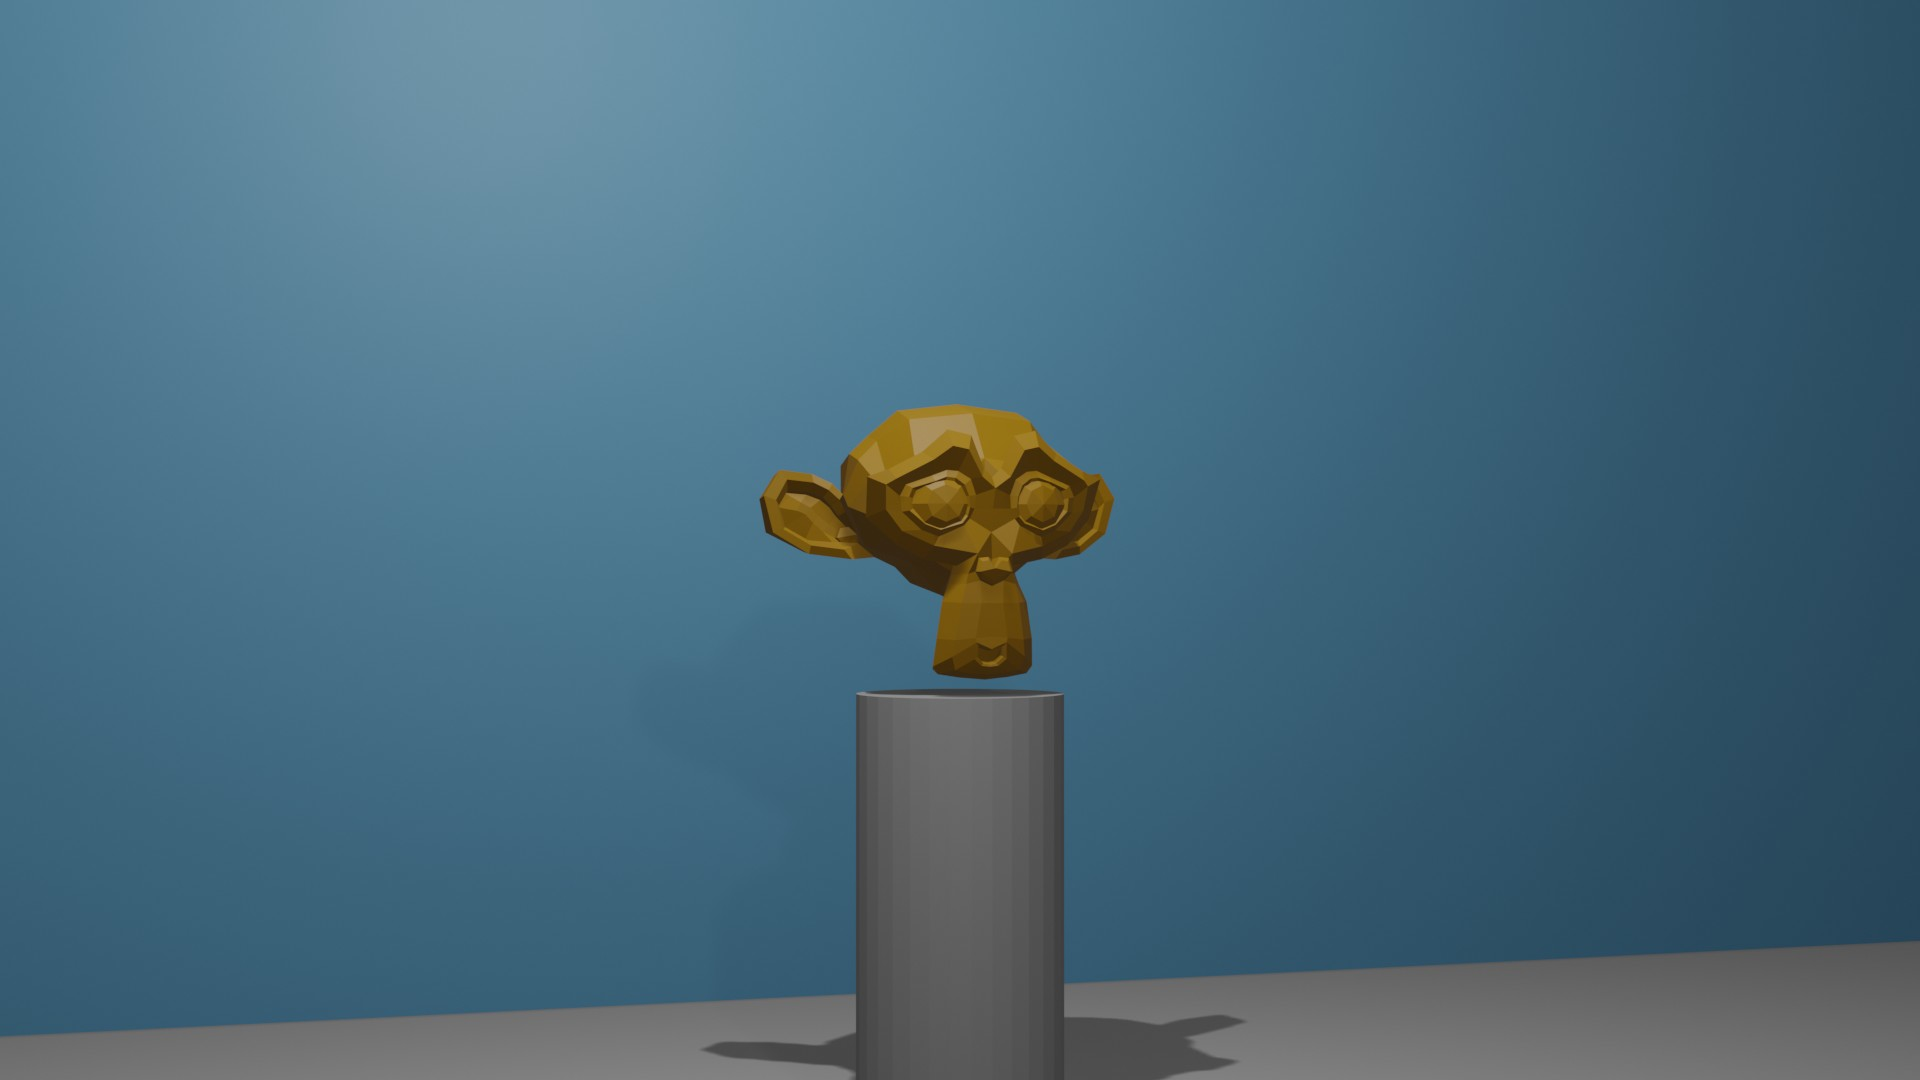
\includegraphics[width=5in]{img/implementation_opencv_original.png}
	\caption{The original render.}	%22_2
	\label{pic:implementation_opencv_original}
\end{figure}

\subsection{Greyscale}
[TODO: Input zweidimensionale Matrix statt dreidimensional (eine Zahl statt 3 pro Pixel)]

\begin{figure}[h!]
	\centering
	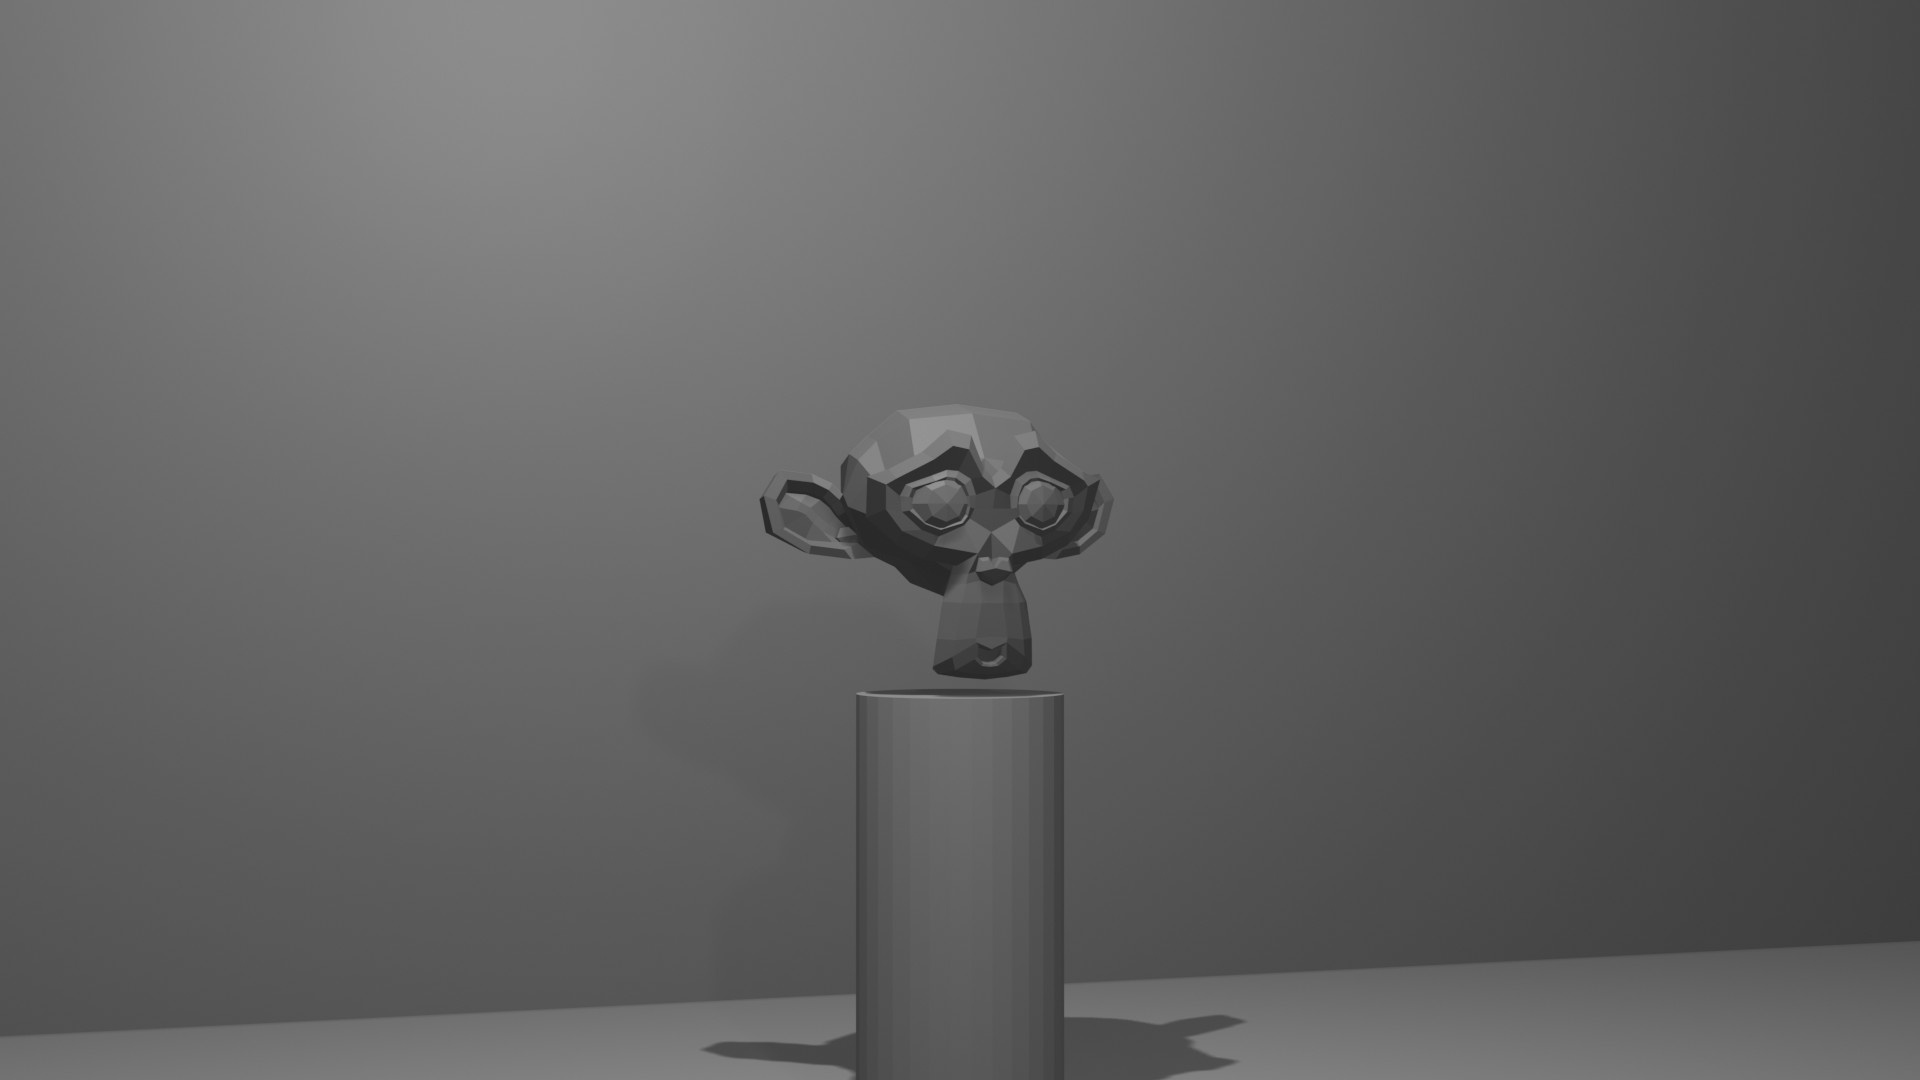
\includegraphics[width=5in]{img/implementation_opencv_greyscale.png}
	\caption{The greyscale image.}
	\label{pic:implementation_opencv_greyscale}
\end{figure}

\subsection{Saturated}

\begin{figure}[h!]
	\centering
	%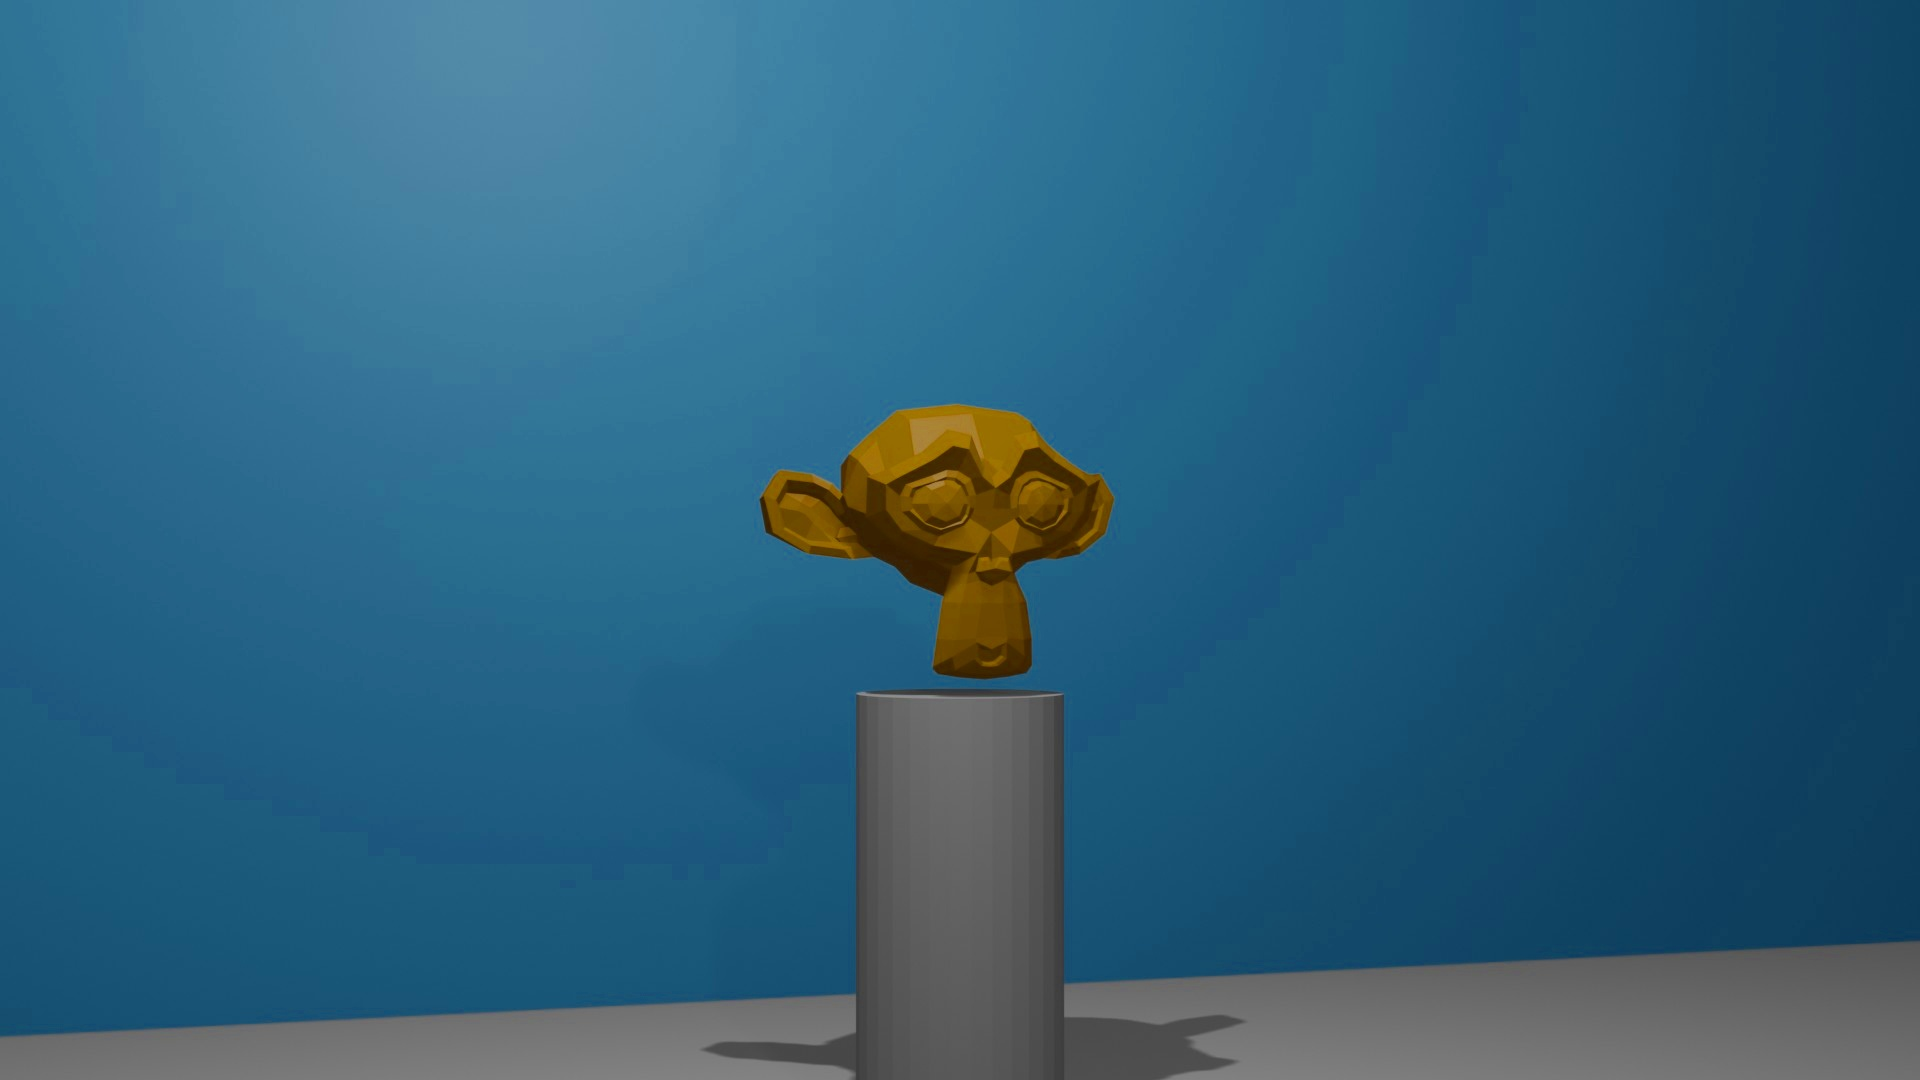
\includegraphics[width=4.5in]{img/implementation_opencv_saturated.png}
	\caption{Comparison between normal and saturated image.}
	\label{pic:implementation_opencv_saturated}
\end{figure}

\subsection{Resolution}

\begin{figure}[h!]
	\centering
	%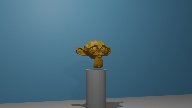
\includegraphics[width=4.5in]{img/implementation_opencv_resolution.png}
	\caption{Comparison between normal and resolution image.}
	\label{pic:implementation_opencv_resolution}
\end{figure}

\subsection{Brightness}

\begin{figure}[h!]
	\centering
	%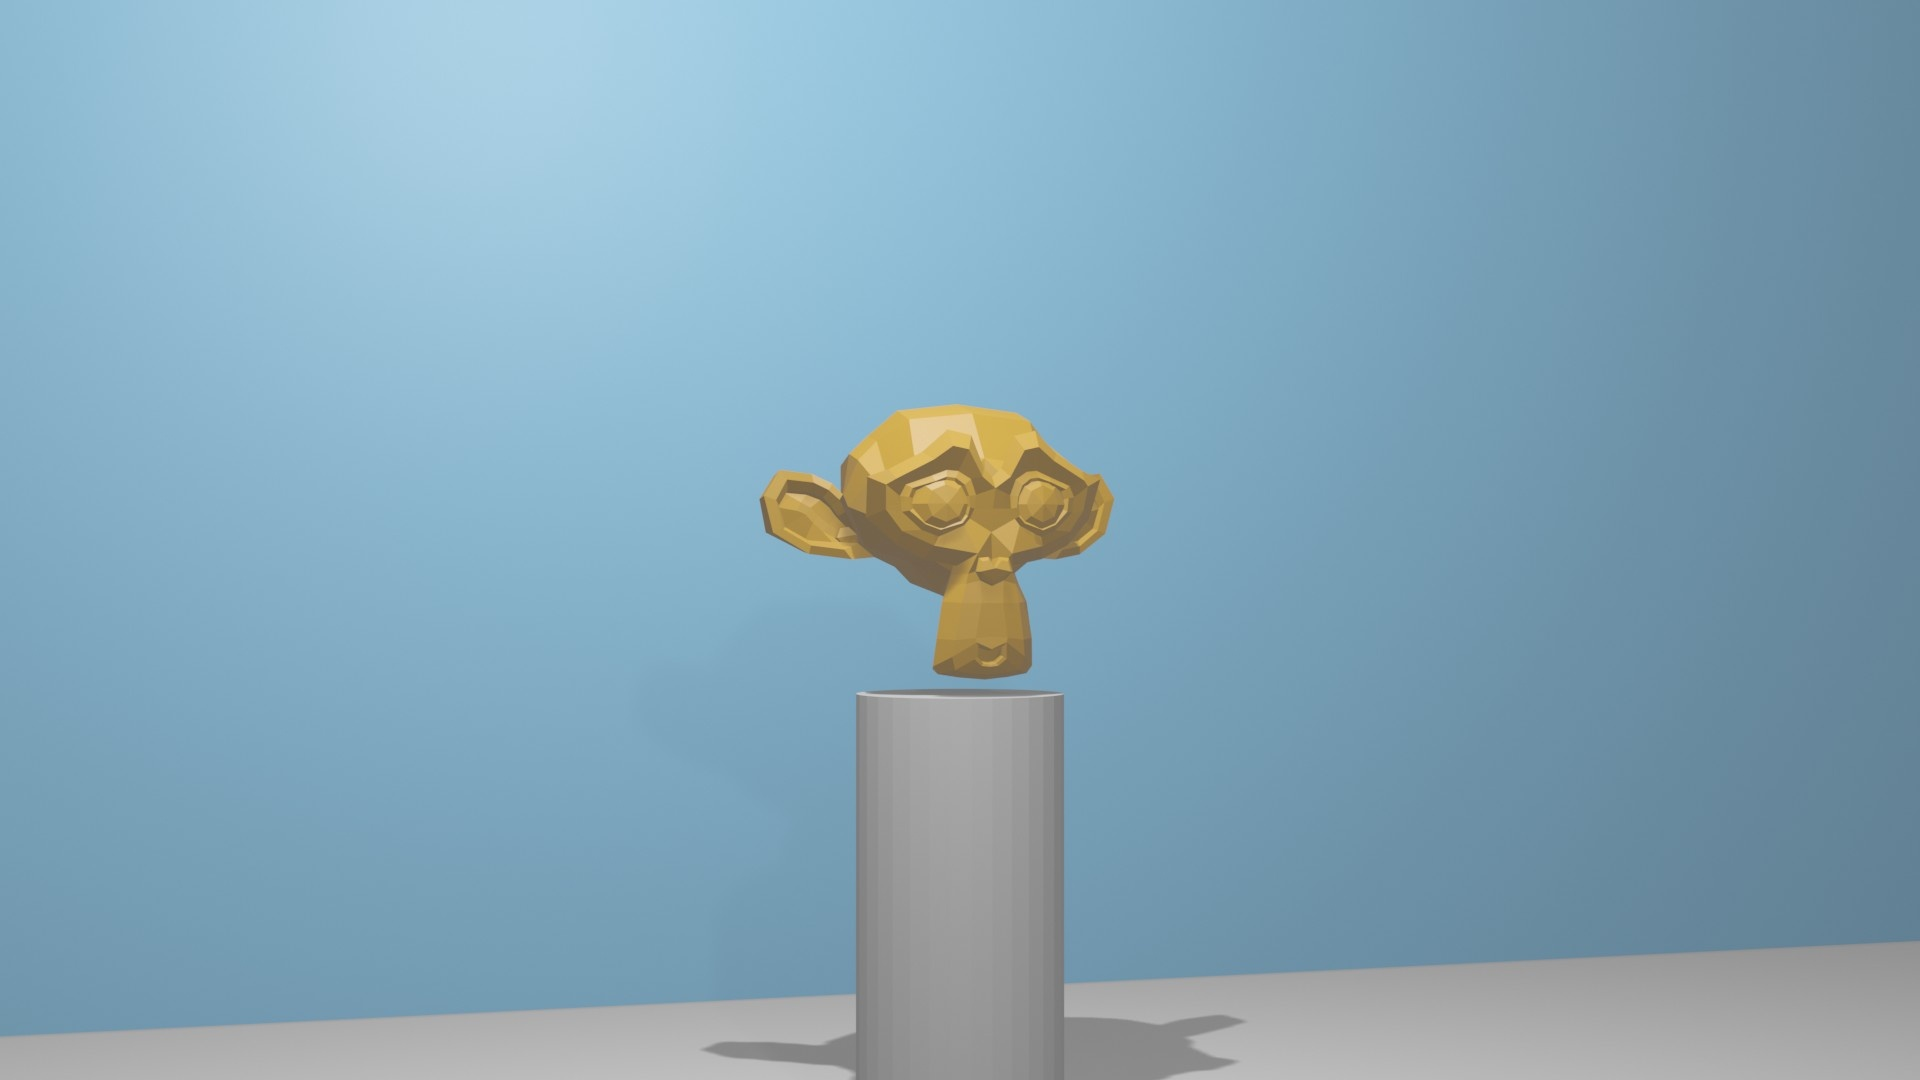
\includegraphics[width=4.5in]{img/implementation_opencv_brightness.png}
	\caption{Comparison between normal and brightness image.}
	\label{pic:implementation_opencv_brightness}
\end{figure}

\section{Neural Network}
\subsection{Structure of our Neural Network}

[wie lesen wir Daten ein, wie viele layer, was ist der output (maximale entfernung? z.B. 10m)]

\section{C++ Implementation}

\section{Technical difficulties}

\filbreak